% Options for packages loaded elsewhere
\PassOptionsToPackage{unicode}{hyperref}
\PassOptionsToPackage{hyphens}{url}
\PassOptionsToPackage{dvipsnames,svgnames*,x11names*}{xcolor}
%
\documentclass[
  12pt,
  ,
  a4paper]{article}
\usepackage{lmodern}
\usepackage{amssymb,amsmath}
\usepackage{ifxetex,ifluatex}
\ifnum 0\ifxetex 1\fi\ifluatex 1\fi=0 % if pdftex
  \usepackage[T1]{fontenc}
  \usepackage[utf8]{inputenc}
  \usepackage{textcomp} % provide euro and other symbols
\else % if luatex or xetex
  \usepackage{unicode-math}
  \defaultfontfeatures{Scale=MatchLowercase}
  \defaultfontfeatures[\rmfamily]{Ligatures=TeX,Scale=1}
\fi
% Use upquote if available, for straight quotes in verbatim environments
\IfFileExists{upquote.sty}{\usepackage{upquote}}{}
\IfFileExists{microtype.sty}{% use microtype if available
  \usepackage[]{microtype}
  \UseMicrotypeSet[protrusion]{basicmath} % disable protrusion for tt fonts
}{}
\makeatletter
\@ifundefined{KOMAClassName}{% if non-KOMA class
  \IfFileExists{parskip.sty}{%
    \usepackage{parskip}
  }{% else
    \setlength{\parindent}{0pt}
    \setlength{\parskip}{6pt plus 2pt minus 1pt}}
}{% if KOMA class
  \KOMAoptions{parskip=half}}
\makeatother
\usepackage{xcolor}
\IfFileExists{xurl.sty}{\usepackage{xurl}}{} % add URL line breaks if available
\IfFileExists{bookmark.sty}{\usepackage{bookmark}}{\usepackage{hyperref}}
\hypersetup{
  pdftitle={Rapport},
  pdfauthor={Alain Quartier-la-Tente},
  pdflang={english},
  colorlinks=true,
  linkcolor=Maroon,
  filecolor=Maroon,
  citecolor=Blue,
  urlcolor=blue,
  pdfcreator={LaTeX via pandoc}}
\urlstyle{same} % disable monospaced font for URLs
\usepackage[margin=1in]{geometry}
\usepackage{longtable,booktabs}
% Correct order of tables after \paragraph or \subparagraph
\usepackage{etoolbox}
\makeatletter
\patchcmd\longtable{\par}{\if@noskipsec\mbox{}\fi\par}{}{}
\makeatother
% Allow footnotes in longtable head/foot
\IfFileExists{footnotehyper.sty}{\usepackage{footnotehyper}}{\usepackage{footnote}}
\makesavenoteenv{longtable}
\usepackage{graphicx,grffile}
\makeatletter
\def\maxwidth{\ifdim\Gin@nat@width>\linewidth\linewidth\else\Gin@nat@width\fi}
\def\maxheight{\ifdim\Gin@nat@height>\textheight\textheight\else\Gin@nat@height\fi}
\makeatother
% Scale images if necessary, so that they will not overflow the page
% margins by default, and it is still possible to overwrite the defaults
% using explicit options in \includegraphics[width, height, ...]{}
\setkeys{Gin}{width=\maxwidth,height=\maxheight,keepaspectratio}
% Set default figure placement to htbp
\makeatletter
\def\fps@figure{htbp}
\makeatother
\setlength{\emergencystretch}{3em} % prevent overfull lines
\providecommand{\tightlist}{%
  \setlength{\itemsep}{0pt}\setlength{\parskip}{0pt}}
\setcounter{secnumdepth}{5}
%début contraintes ensae
\usepackage{pdfpages, setspace, mathptmx} %times roman
\usepackage{textpos}%pour textblock
\onehalfspacing 
\definecolor{rougeENSAE}{RGB}{188, 24, 39}

\makeatletter
%CREDITS : @antuki
\def\@maketitle{%
  \clearpage
 \thispagestyle{empty}

\begin{textblock*}{\textwidth}(-7cm,-3.5cm)
\begin{center}

\includegraphics[height=3cm]{img/900px-LOGO-ENSAE.png}
\end{center}
\end{textblock*}

\begin{minipage}{0.4\textwidth}
  \begin{flushleft} \large
    \textbf{Alain \textsc{Quartier-la-Tente} \vspace{8.75mm} }
  \end{flushleft}
\end{minipage}
\begin{minipage}{0.6\textwidth}
  \begin{flushright} 
  \large{
    \textbf{ENSAE 2\textsuperscript{ème} année\\}
  }     
  \small
    \textbf{ 
        \textit{Stage d'application\\
        Année scolaire 2019 - 2020}
    }
  \end{flushright}
\end{minipage}

\vspace*{5cm}

\begin{center}
    \fbox{\parbox{0.9\textwidth}{
        \begin{huge}\begin{center}
        \textbf{Real-time detection of turning points with linear filters}\\
        
        %\textbf{Détection en temps réel des points de retournement}\\
        \end{center}\end{huge}}}
\end{center}

\vfill
    
\begin{minipage}{0.5\textwidth}
    \begin{flushleft} \large 
    \textbf{Banque Nationale de Belgique\\
        Cellule Recherche et Développement
    }
  \end{flushleft}
\end{minipage} 
\begin{minipage}{0.5\textwidth}
  \begin{flushright} \large
    \textbf{
        Maître de stage : Jean \textsc{Palate}\\
        08/06/2020 - 14/08/2020
    }
  \end{flushright}
\end{minipage}    

\vspace*{1cm}


\textcolor{rougeENSAE}{\rule{10mm}{1.5mm}}

\scriptsize
\textbf{ENSAE Paris}\newline TSA 26644
\rightline{\href{www.ensae.fr}{\textcolor{rougeENSAE}{\textbf{www.ensae.fr}}}$\quad \qquad \qquad$}

Service des relations entreprises et des stages\newline
5, avenue Henry Le Chatelier -- 91764 PALAISEAU CEDEX -- FRANCE -- Tél : +33 (0)1 70 26 67 39 -- Courriel : stage\symbol{64}ensae.fr

\normalsize

\clearpage
\setcounter{page}{0}
}

\makeatother% cinsérer page de garde

\usepackage{stmaryrd}
\usepackage{multicol}
\usepackage{graphicx}
\usepackage{animate, dsfont, here, xspace}
%\usepackage{tikz}       
\usepackage{tikz,pgfplots}
 \pgfplotsset{compat=1.17}
%
\includepdf[fitpaper=true, pages=-]{img/pdg.pdf}


\DeclareMathOperator{\e}{e}
\renewcommand{\P}{\mathds{P}} %Apparement \P existe déjà ?
\newcommand\N{\mathds{N}}
\newcommand\R{\mathds{R}}
%\newcommand\C{\mathds{C}}
%\newcommand\Z{\mathds{Z}}


\newcommand\1{\mathds{1}}
\newcommand{\E}[2][]{{\mathds{E}}_{#1}
  \def\temp{#2}\ifx\temp\empty
  \else
    \left[#2\right]
  \fi
}
\newcommand{\V}[2][]{{\mathds{V}}_{#1}
  \def\temp{#2}\ifx\temp\empty
  \else
    \left[#2\right]
  \fi
}
\newcommand\ud{\,\mathrm{d}}

% blocks
\usepackage{environ}
\usepackage[tikz]{bclogo}

\tikzstyle{titlestyle} =[draw=black!80,fill=black!20, text=black,
 right=10pt, rounded corners]
\mdfdefinestyle{symmaryboxstyle}{
	linecolor=black!80, backgroundcolor = black!5,
	skipabove=\baselineskip, innertopmargin=\baselineskip,
	innerbottommargin=\baselineskip,
	userdefinedwidth=\textwidth,
	middlelinewidth=1.2pt, roundcorner=5pt,
	skipabove={\dimexpr0.5\baselineskip+\topskip\relax},
	frametitleaboveskip=\dimexpr-\ht\strutbox\relax,
	innerlinewidth=0pt,
}
\NewEnviron{summary}[2][true]{%
\begin{mdframed}[style=symmaryboxstyle,
nobreak=#1,
frametitle={%
      \tikz[baseline=(current bounding box.east),outer sep=0pt]
      \node[titlestyle,anchor=east]
    {Summary --- #2};}
]
\vspace{-0.5em}
\BODY
\end{mdframed}
}

\usepackage{amsthm}
%\theoremstyle{remark}
\newtheorem*{remark}{Remark}

\usepackage{mathrsfs}
\usepackage{fontawesome5}
\usepackage{booktabs}
\usepackage{longtable}
\usepackage{array}
\usepackage{multirow}
\usepackage{wrapfig}
\usepackage{float}
\usepackage{colortbl}
\usepackage{pdflscape}
\usepackage{tabu}
\usepackage{threeparttable}
\usepackage{threeparttablex}
\usepackage[normalem]{ulem}
\usepackage{makecell}
\usepackage{xcolor}
\ifxetex
  % Load polyglossia as late as possible: uses bidi with RTL langages (e.g. Hebrew, Arabic)
  \usepackage{polyglossia}
  \setmainlanguage[]{}
\else
  \usepackage[shorthands=off,main=]{babel}
\fi
\usepackage[style=authoryear,]{biblatex}
\addbibresource{biblio.bib}

\title{Rapport}
\author{Alain Quartier-la-Tente}
\date{6/17/2020}

\begin{document}
\maketitle

{
\hypersetup{linkcolor=}
\setcounter{tocdepth}{3}
\tableofcontents
}
\newpage

\hypertarget{abstract}{%
\section{Abstract}\label{abstract}}

\newpage

\hypertarget{introduction}{%
\section{Introduction}\label{introduction}}

With the COVID-19 crisis, one of the major question on the economy was when it will collapse and when it will recover.
It illustrates that business cycle analysis, and in particular the early detection of turning points in a series, is a major topic in the analysis of economic outlook.
Moving averages, or linear filters, are ubiquitous in business cycle extraction and seasonal adjustment methods\footnote{A moving average is a statistical method that consists in applying a rolling weighted mean to a times series: for each date it computes a weighted mean of \(p\) past points and \(q\) future points where \(p,q\geq0\) depends on the moving average.}.
For example, the X-12ARIMA seasonal adjustment method uses Henderson moving averages and composite moving averages to estimate the main components of a time series, while TRAMO-SEATS uses Wiener-Kolmogorov filters.
Symmetric filters are applied to the center of the series, but when it comes to estimate the most recent points, all of these methods must rely on asymmetric filters.
For example, X-12ARIMA or TRAMO-SEATS apply symmetrical averages to the forecasts obtained from an ARIMA model of the series.
However, since the predicted values are linear combinations of past values, it consist in applying to use methods do use skewed moving averages at the end of the series.

If the classic asymmetric moving averages have good properties regarding the size of future revisions induces by the process\footnote{See for example \textcite{pierce1980SA}.}, they induce phase shifts that impact the real-time estimation of turning points, introducing time delay in the detection.

This report aims to describe and compare the recent approaches around trend-cycle extraction and asymmetric filters.
Due to the link between seasonal adjustment and trend-cycle extraction (section \ref{sec:SAtoTCE}), we here focus on non-parametric methods that could be included in X-12ARIMA.
After a description of the general properties link between seasonal adjustment and trend-cycle estimation (\ref{sec:SAtoTCE}), we described the linear filters methods developed by \textcite{proietti2008}, \textcite{ch15HBSA}, \textcite{trilemmaWMR2019} and \textcite{dagumbianconcini2008} (sections \ref{sec:lppfilters} to @ref(sec:Dagum\}).

\newpage

\hypertarget{sec:SAtoTCE}{%
\section{From seasonal adjustment to trend-cycle estimation}\label{sec:SAtoTCE}}

Since the 20th century, more and more infra-annual statistics are produced, especially by national institutes, to analyse the short-term evolution of economies.
It is for example the case of the gross domestic product (GDP), unemployment rate, household consumption of goods and industrial production indices.
However, most of those time series are affected by seasonal and trading days effects.
A seasonal effect is an effect that occurs in the same calendar month with similar magnitude and direction from year to year.
For instance, automobile production is usually lower during summer, due to holidays, and chocolate sales are usually higher in December, due to Christmas.
Trading days effect appears when a time series is affected by calendar month's weekday composition.
For example retail sales are usually higher on Saturday, thus it is likely that they will be higher in months with a surplus of weekend days.

Seasonal and trading days effects can hamper the analysis of infra-annual movements of a time series or the spatial comparison.
This is the reason why time series are often seasonally and trading days adjusted, where seasonal adjustment is the process of removing the effects of seasonal and trading day fluctuations.

To perform seasonal adjustment, most of the algorithm decompose the data in several unknown component: trend-cycle, seasonal and irregular component.
In X-12ARIMA and TRAMO-SEATS (the most popular seasonal adjustment methods), prior to the decomposition, the initial series is pre-adjustment from deterministic effects (outliers, calendar effects).
Thus, the estimation of trend-cycle component technically is linked to the seasonal component.

Moreover, since the trend-cycle extraction methods are applied to seasonally adjusted data, both problem cannot be separated.
This link also explains that in this paper, all the methods used are implemented in the core libraries of JDemetra+ \footnote{\url{https://github.com/jdemetra/jdemetra-core}.}, the seasonal adjustment software recommended by Eurostat.
An \faIcon{r-project} interface is implemented in the package \texttt{rjdfilters}\footnote{\url{https://github.com/palatej/rjdfilters}.} was developped during this internship.

In this paper we focus methods that could be implemented in X-12ARIMA.
To maintain consistency with the non-parametric approach of X-12ARIMA, we focus on non-parametric extraction methods.
That's why the filters of the approach of \textcite{trilemmaWMR2019} (section~\ref{sec:WildiMcLeroy}) are described but not used in this report.

Furthermore, for simplicity the data used is seasonally adjusted: the study should be extended to see the impact on the overall seasonal adjustment process.

\hypertarget{sec:propMM}{%
\section{Moving average and filters}\label{sec:propMM}}

A lot of papers describes the definition and the properties of moving average and linear filters (see for example \textcite{ch12HBSA}).
Here we summarize some of the main results.

Let \(p\) et \(f\) two integers, a moving average \(M_\theta\) or \(M\) is defined by a set of coefficients \(\theta=(\theta_{-p},\dots,\theta_{f})'\) such as:
\[
M_\theta(X_t)=\sum_{k=-p}^{+f}\theta_kX_{t+k}
\]

\begin{itemize}
\item
  \(p+f+1\) is called the \emph{moving average order}.
\item
  When \(p=f\) the moving average is said to be \emph{centered}.
  If we also have \(\forall k:\:\theta_{-k} = \theta_k\), the moving average \(M_\theta\) is said to be \emph{symmetric}.
  In this case, the quantity \(h=p=f\) is called the \emph{bandwidth}.
\end{itemize}

\hypertarget{gain-and-phase-shift-functions}{%
\subsection{Gain and phase shift functions}\label{gain-and-phase-shift-functions}}

Let \(X_t=\e^{-i\omega t}\), the result of the moving average \(M_\theta\) in \(X_t\) is:
\[
Y_t = M_{\theta}X_t = \sum_{k=-p}^{+f} \theta_k \e^{-i \omega (t+k)}
= \left(\sum_{k=-p}^{+f} \theta_k \e^{-i \omega k}\right)\cdot X_t.
\]
The function \(\Gamma_\theta(\omega)=\sum_{k=-p}^{+f} \theta_k e^{-i \omega k}\) is called the \emph{transfer function} or \emph{frequency response function}\footnote{The frequency response function can equivalently be defined as \(\Gamma_\theta(\omega)=\sum_{k=-p}^{+f} \theta_k e^{i \omega k}\) or \(\Gamma_\theta(\omega)=\sum_{k=-p}^{+f} \theta_k e^{2\pi i \omega k}\).}.
It can be rewritten as:
\[
\Gamma_\theta(\omega) = G_\theta(\omega)\e^{-i\Phi_\theta(\omega)}
\]
where \(G_\theta(\omega)=\lvert\Gamma_\theta(\omega)\rvert\) is the \emph{gain} or \emph{amplitude} function and \(\Phi_\theta(\omega)\) is the \emph{phase shift} or \emph{time shift} function\footnote{This function is sometimes represented as \(\phi_\theta(\omega)=\frac{\Phi_\theta(\omega)}{\omega}\) to mesure the phase shift in number of periods.}.
For all symmetric moving average we have \(\Phi_\theta(\omega)\equiv 0 \pmod{\pi}\).

To sum up, applying a moving average to an harmonic times series affects in in two different ways:

\begin{itemize}
\item
  by multiplying it by an amplitude coefficient \(G_{\theta}\left(\omega\right)\);
\item
  by ``shifting'' it in time by \(\Phi_\theta(\omega)/\omega\), which directly affects the detection of turning points\footnote{When \(\Phi_\theta(\omega)/\omega>0\) the time shift is positive: a turning point is detected with delay.}.
\end{itemize}

Example: with \(M_{\theta_0}X_t=\frac{1}{2}X_{t-1}+\frac{1}{2}X_{t}\) we have:
\[
\Gamma_{\theta_0}(\omega)=\frac{1}{2}+\frac{1}{2}\e^{-i\omega}
=\lvert\cos(\omega/2)\rvert\e^{-i\frac{\omega}{2}}
\]
The figure \ref{fig:exgainPhase} illustrates the gain and the phase shift for \(\omega=\pi/2\) and \(X_t=\sin(\omega t)\).

\begin{figure}[!ht]
\pgfplotsset{width=\textwidth,height=6cm,every axis legend/.append style={font=\footnotesize,
  at={(0.5,-0.1)},
  anchor=north}
    }
\begin{tikzpicture}
\begin{axis}[
legend columns=2,
legend style = {fill=none , fill opacity=0, draw opacity=1,text opacity=1},
xtick={0,3.14159,...,15.70795},
xticklabels={0,$\pi$,$2\pi$,$3\pi$,$4\pi$,$5\pi$} 
]
\addplot[domain=0:5*pi,smooth,samples=300]    plot (\x,{sin(\x * (pi/2) r)});
\addlegendentry{$X_t(\pi/2)$}
\addplot[domain=0:5*pi,smooth,samples=300, dashed]    
  plot (\x,{1/2*sin(\x* pi/2 r )+1/2*sin((\x -1) * pi/2 r)});
\addlegendentry{$M_{\theta_0}X_t(\pi/2)$}
\draw[<->](axis cs: 1.5,1)--(axis cs: 1.5,0.7071068)
  node[pos=0.5, right]{\scriptsize $G_{\theta_0}(\pi/2)$};
\draw[<->] (axis cs: 3, -0.70710680-0.05)--(axis cs: 3.5,-0.7071068-0.05) 
  node[pos=0.5, below right]{\scriptsize $\Phi_{\theta_0}(\pi/2)$};
\end{axis}
\end{tikzpicture}
\caption{Smoothing of the time series $X_t=\sin(\omega t)$ by the moving average $M_{\theta_0}X_t=\frac{1}{2}X_{t-1}+\frac{1}{2}X_{t}$ for $\omega=\pi/2$.}\label{fig:exgainPhase}
\end{figure}

\hypertarget{desirable-properties-of-a-moving-average}{%
\subsection{Desirable properties of a moving average}\label{desirable-properties-of-a-moving-average}}

The moving average are often constructed under some specific constraints.
In the report we will focus on two constraints:

\begin{itemize}
\item
  the preservation of certain kind of trends;
\item
  the variance reduction.
\end{itemize}

\hypertarget{trend-preservation}{%
\subsubsection{Trend preservation}\label{trend-preservation}}

It is often desirable for a moving average to conserve certain kind of trends.
A moving average \(M_\theta\) conserve a function of the time \(f(t)\) if \(\forall t:\:M_\theta f(t)=f(t)\).

We have the following properties for the moving average \(M_\theta\):

\begin{itemize}
\item
  To conserve a constant series \(X_t=a\) we need
  \[
  \forall t:M_\theta(X_t)=\sum_{k=-p}^{+f}\theta_kX_{t+k}=\sum_{k=-p}^{+f}\theta_ka=a\sum_{k=-p}^{+f}\theta_k=a
  \]
  the sum of the coefficients of the moving average \(\sum_{k=-p}^{+f}\theta_k\) must then be equal to \(1\).
\item
  To conserve a linear trend \(X_t=at+b\) we need:
  \[
  \forall t:\:M_\theta(X_t)=\sum_{k=-p}^{+f}\theta_kX_{t+k}=\sum_{k=-p}^{+f}\theta_k[a(t+k)+b]=at\sum_{k=-p}^{+f}k\theta_k+b\sum_{k=-p}^{+f}\theta_k=at+b
  \]
  which is equivalent to:
  \[
  \sum_{k=-p}^{+f}\theta_k=1
  \quad\text{and}\quad
  \sum_{k=-p}^{+f}k\theta_k=0
  \]
\item
  In general, it can be shown that \(M_\theta\) conserve a polynomial of degree \(d\) if and only if:
  \[
  \sum_{k=-p}^{+f}\theta_k=1 
   \text{ and } 
  \forall j \in \left\llbracket 1,d\right\rrbracket:\:
  \sum_{k=-p}^{+f}k^j\theta_k=0
  \]
\item
  If \(M_\theta\) is symmetric (\(p=f\) and \(\theta_{-k} = \theta_k\)) and conserve polynomial of degree \(2d\) then it also conserve polynomial of degree \(2d+1\).
\end{itemize}

\hypertarget{variance-reduction}{%
\subsubsection{Variance reduction}\label{variance-reduction}}

All time series are affected by noise that can blur the signal extraction.
Hence, we seek to reduce the variance of the noise.
The sum of the sum of the squares of the coefficients \(\sum_{k=-p}^{+f}\theta_k^2\) is the \emph{variance reduction} ratio.

Indeed, let \(\{\varepsilon_t\}\) a sequence of independent random variables with \(\E{\varepsilon_t}=0\), \(\V{\varepsilon_t}=\sigma^2\).
\[
\V{M_\theta\varepsilon_t}=\V{\sum_{k=-p}^{+f} \theta_k \varepsilon_{t+k}}
= \sum_{k=-p}^{+f} \theta_k^2 \V{\varepsilon_{t+k}}=
\sigma^2\sum_{k=-p}^{+f} \theta_k^2
\]

\hypertarget{defAsymProb}{%
\subsection{Real-time estimation and asymmetric moving average}\label{defAsymProb}}

For symmetric filters, the phase shift function is equal to zero.
Therefore, there is no delay in any frequency: that's why they are prefered to the asymmetric ones.
However, they cannot be used in the beginning and in the end of the time series because no past/future value can be used.
Thus, for real-time estimation, it is needed to build asymmetric moving average that approximate the symmetric moving average.

The approximation is summarised by quality indicators.
In this paper we focus on the ones defined by \textcite{ch15HBSA} and \textcite{trilemmaWMR2019} to build the asymmetric filters.

\textcite{ch15HBSA} propose a general approach to derive linear filters, based on an optimization problem of three criteria: \emph{Fidelity} (\(F_g\), noise reduction), \emph{Smoothness} (\(S_g\)) and \emph{Timeliness} (\(T_g\), phase shift between input and ouput signals).
See section \ref{sec:GuggemosEtAl} for more details.

\textcite{trilemmaWMR2019} propose an approach based on the decomposition of the mean squared error between the symmetric and the asymmetric filter in four quantities: \emph{Accuracy} (\(A_w\)), \emph{Timeliness} (\(T_w\)), \emph{Smoothness} (\(S_w\)) and \emph{Residual} (\(R_w\)).
See section \ref{sec:WildiMcLeroy} for more details.

All the indicators are summarized in table \ref{tab:QC}.

\begin{table}[!ht]
$$\begin{array}{ccc}
\hline \text{Sigle} & \text{Description} & \text{Formula}\\
\hline b_{c} & \text{constant bias} & \sum_{k=-p}^{+f}\theta_{k}-1\\
\hline b_{l} & \text{linear bias} & \sum_{k=-p}^{+f}k\theta_{k}\\
\hline b_{q} & \text{quadratic bias} & \sum_{k=-p}^{+f}k^{2}\theta_{k}\\
\hline F_{g} & \text{variance reduction / fidelity} & \sum_{k=-p}^{+f}\theta_{k}^{2}\\
\hline S_{g} & \text{Smoothness (Guggemos)} & \sum_{j}(\nabla^{3}\theta_{j})^{2}\\
\hline T_{g} & \text{Timeliness (Guggemos)} & \int_{0}^{2\pi/12}\rho_{\theta}(\omega)\sin(\varphi_{\theta}(\omega))^{2}\ud\omega\\
\hline A_{w} & \text{Accuracy (Wildi)} & 2\int_0^{2\pi/12}\left(\rho_{s}(\omega)-\rho_{\theta}(\omega)\right)^{2}h_{RW}(\omega)\ud\omega\\
\hline T_{w} & \text{Timeliness (Wildi)} & 8\int_0^{2\pi/12} \rho_{s}(\omega)\rho_{\theta}(\omega)\sin^{2}\left(\frac{\varphi_\theta(\omega)}{2}\right)h_{RW}(\omega)\ud\omega\\
\hline S_{w} & \text{Smoothness (Wildi)} & 2\int_{2\pi/12}^{\pi}\left(\rho_{s}(\omega)-\rho_{\theta}(\omega)\right)^{2}h_{RW}(\omega)\ud\omega\\
\hline R_{w} & \text{Residual (Wildi)} & 8\int_{2\pi/12}^{\pi} \rho_{s}(\omega)\rho_{\theta}(\omega)\sin^{2}\left(\frac{\varphi_\theta(\omega)}{2}\right)h_{RW}(\omega)\ud\omega\\
\hline \\
\end{array} $$
\caption{Criteria used to check the quality of a linear filter defined by its coefficients $\theta=(\theta_k)_{-p\leq k\leq f}$ and its gain and phase shift function, $\rho_{\theta}$ and $\varphi_\theta$.} 
\label{tab:QC}
\footnotesize
\emph{Note: $X_g$ criteria are derived from \textcite{ch15HBSA} and $X_w$ criteria from \textcite{trilemmaWMR2019}.}

\emph{$\rho_s$ represent the gain function of an Henderson symmetric filter to compare with the asymmetric ones.}

\emph{$h_{RW}$ is the spectral density of a random walk: $h_{RW}(\omega)=\frac{1}{2(1-\cos(\omega))}$.}
\end{table}

\hypertarget{sec:lppfilters}{%
\section{Local polynomial filters}\label{sec:lppfilters}}

In this section we detail the filters that arised from fitting a local polynomial to our time series, as described by \textcite{proietti2008}.

We assume that our time series \(y_t\) can be decomposed as
\[
y_t=\mu_t+\varepsilon_t
\]
where \(\mu_t\) is the signal (trend) and \(\varepsilon_{t}\overset{i.i.d}{\sim}\mathcal{N}(0,\sigma^{2})\) is the noise\footnote{The time series is therefore seasonnally adjusted}.
We assume that \(\mu_t\) can be locally approximated by a polynomial of degree \(d\) of the time \(t\) between \(y_t\) and the neighboring observations \(\left(y_{t+j}\right)_{j\in\left\llbracket -h,h\right\rrbracket}\). Then \(\mu_t\simeq m_{t}\) with:
\[
\forall j\in\left\llbracket -h,h\right\rrbracket :\:
y_{t+j}=m_{t+j}+\varepsilon_{t+j},\quad m_{t+j}=\sum_{i=0}^{d}\beta_{i}j^{i}
\]
This signal extraction problem is then equivalent to the estimation of \(m_t=\beta_0\). In matrix notation we can write:
\[
\underbrace{\begin{pmatrix}y_{t-h}\\
y_{t-(h-1)}\\
\vdots\\
y_{t}\\
\vdots\\
y_{t+(h-1)}\\
y_{t+h}
\end{pmatrix}}_{y}=\underbrace{\begin{pmatrix}1 & -h & h^{2} & \cdots & (-h)^{d}\\
1 & -(h-1) & (h-1)^{2} & \cdots & (-(h-1))^{d}\\
\vdots & \vdots & \vdots & \cdots & \vdots\\
1 & 0 & 0 & \cdots & 0\\
\vdots & \vdots & \vdots & \cdots & \vdots\\
1 & h-1 & (h-1)^{2} & \cdots & (h-1)^{d}\\
1 & h & h^{2} & \cdots & h^{d}
\end{pmatrix}}_{X}\underbrace{\begin{pmatrix}\beta_{0}\\
\beta_{1}\\
\vdots\\
\vdots\\
\vdots\\
\vdots\\
\beta_{d}
\end{pmatrix}}_{\beta}+\underbrace{\begin{pmatrix}\varepsilon_{t-h}\\
\varepsilon_{t-(h-1)}\\
\vdots\\
\varepsilon_{t}\\
\vdots\\
\varepsilon_{t+(h-1)}\\
\varepsilon_{t+h}
\end{pmatrix}}_{\varepsilon}
\]
Two parameters are crucial in determining the accuracy of the approximation:

\begin{itemize}
\item
  the degree \(d\) of the polynomial;
\item
  the number of neighboured \(H=2h+1\) (or the \emph{bandwidth} \(h\)).
\end{itemize}

In order to estimate \(\beta\) we need \(H\geq d+1\) and the estimation is done by the weighted least squares (WLS), which consists of minimizing the following objective function:
\[
S(\hat{\beta}_{0},\dots,\hat{\beta}_{d})=\sum_{j=-h}^{h}\kappa_{j}(y_{t+j}-\hat{\beta}_{0}-\hat{\beta}_{1}j-\dots-\hat{\beta}_{d}j^{d})^{2}
\]
where \(\kappa_j\) is a set of weights called \emph{kernel}. We have \(\kappa_j\geq 0\), \(\kappa_{-j}=\kappa_j\) and with \(K=diag(\kappa_{-h},\dots,\kappa_{h})\), the estimate of \(\beta\) can be written as \(\hat{\beta}=(X'KX)^{1}X'Ky\).
With \(e_{1}=\begin{pmatrix}1&0&\cdots&0\end{pmatrix}'\), the estimate of the trend is:
\[
\hat{m}_{t}=e_{1}\hat{\beta}=w'y=\sum_{j=-h}^{h}w_{j}y_{t-j}\text{ with }w=KX(X'KX)^{-1}e_{1}
\]
To conclude, the estimate of the trend \(\hat{m}_{t}\) can be obtained applying the symmetric filter \(w\) to \(y_t\)\footnote{\(w\) is symmetric due to the symmetry of the kernel weights \(\kappa_j\).}.
Moreover, \(X'w=e_{1}\) so:
\[
\sum_{j=-h}^{h}w_{j}=1,\quad\forall r\in\left\llbracket 1,d\right\rrbracket :\sum_{j=-h}^{h}j^{r}w_{j}=0
\]
Hence, the filter \(w\) preserve deterministic polynomial of order \(d\).

\hypertarget{sec:kernels}{%
\subsection{Different kernels}\label{sec:kernels}}

In signal extraction, we generally look for weighting observations according to their distance from time \(t\): this is the role of the kernel function.
For that, we introduce a kernel function \(\kappa_j\), \(j=0,\pm1,\dots,\pm h\) with \(\kappa_j \geq0\) and \(\kappa_j=\kappa_{-j}\).
An important class of kernels is the Beta kernels. In the discrete, up to a proportional factor (so that \(\sum_{j=-h}^h\kappa_j=1\)):
\[
\kappa_j = \left(
  1-
  \left\lvert
  \frac j {h+1}
  \right\lvert^r
\right)^s
\]
with \(r>0\), \(s\geq 0\).
It encompass all kernels used in this report, except Henderson, trapezoidal and gaussian kernel.The following kernels are considered in this report:

\begin{multicols}{2}
\begin{itemize}
\item $r=1,s=0$ uniform kernel: 
$$\kappa_j^U=1$$
\item $r=s=1$ triangle kernel:
$$\kappa_j^T=\left(
  1-
  \left\lvert
  \frac j {h+1}
  \right\lvert
\right)$$

\item $r=2,s=1$  Epanechnikov (or Parabolic) kernel:
$$\kappa_j^E=\left(
  1-
  \left\lvert
  \frac j {h+1}
  \right\lvert^2
\right)$$

\item $r=s=2$ biweight kernel:
$$\kappa_j^{BW}=\left(
  1-
  \left\lvert
  \frac j {h+1}
  \right\lvert^2
\right)^2$$

\item $r = 2, s = 3$ triweight kernel:
$$\kappa_j^{TW}=\left(
  1-
  \left\lvert
  \frac j {h+1}
  \right\lvert^2
\right)^3$$

\item $r = s = 3$ tricube kernel:
$$\kappa_j^{TC}=\left(
  1-
  \left\lvert
  \frac j {h+1}
  \right\lvert^3
\right)^3$$

\item Henderson kernel (see section \ref{sec:sympolyfilter} for more details):
$$
\kappa_{j}=\left[1-\frac{j^2}{(h+1)^2}\right]
\left[1-\frac{j^2}{(h+2)^2}\right]
\left[1-\frac{j^2}{(h+3)^2}\right]
$$
\item Trapezoidal kernel:
$$
\kappa_j^{TP}=
\begin{cases}
  \frac{1}{3(2h-1)} & \text{ if }j=\pm h 
  \\
  \frac{2}{3(2h-1)} & \text{ if }j=\pm (h-1)\\
  \frac{1}{2h-1}& \text{ otherwise}
\end{cases}
$$
\item Gaussian kernel\footnote{
In this report we arbirarily take $\sigma^2=0.25$.
}
$$
\kappa_j^G=\exp\left(
-\frac{
  j^2
}{
  2\sigma^2h^2
}\right)
$$
\end{itemize}
\end{multicols}

Henderson, trapezoidal and gaussian kernel are very specific:

\begin{itemize}
\item
  The kernel Henderson and trapezoidal function change with the bandwidth (the other kernel only depend on the ratio \(j/h+1\)).
\item
  Other definitions of the trapezoidal and gaussian kernel can be used.
  The trapezoidal kernel is here considered because it corresponds to the filter used to extract the seasonal component in the X-12ARIMA algorithm.
  Therefore it is never used to extract trend-cycle component.
\end{itemize}

\begin{figure}[!ht]
\animategraphics[autoplay,loop,width=\textwidth,controls]{2}{img/kernels/}{2}{30} 
\caption{Coefficients of the different kernels for $h$ from 2 to 30.}\label{fig:kernels}\footnotesize
\emph{Note: to see the animation, the PDF must be open with Acrobat Reader, KDE Okular, PDF-XChange or Foxit Reader. 
Otherwise you will only be able to see the results for $h=2$.}
\end{figure}

The figure \ref{fig:kernels} summarises the coefficients of the different kernels.
Analysing the coefficients we can already anticipate some properties of the associated filters:

\begin{itemize}
\item
  The triweight kernel has the narrowest distribution.
  The narrowest a distribution is, the smallest the weights of furthest neighbours are: the associated filter should have a high weight in the current observation (\(t\)).
\item
  For \(h\) high the Henderson kernel is equivalent to the triweight kernel (since \(h+1\sim h+2 \sim h+3\), \(\kappa_j^H\sim\kappa_j^{TW}\)), the associated filter should also be equivalent.
  However, for \(h\) small (\(h\leq10\)) the Henderson kernel is closer to the biweight kernel than to the triweight kernel.
\end{itemize}

\hypertarget{sec:sympolyfilter}{%
\subsubsection{Specific symmetric filters}\label{sec:sympolyfilter}}

When \(p=0\) (local adjustment by a constant) we obtain the \textbf{Nadaraya-Watson}'s estimator.

With the uniform kernel we obtain the \textbf{Macaulay filter}. When \(p=0,1\), this is the arithmetic moving average: \(w_j=w=\frac{1}{2h+1}\).

The \textbf{Epanechnikov} kernel is often recommended as the optimal kernel that minimize the mean square error of the estimation by local polynomial.

\textbf{Loess} is a locally weighted polynomial regression that use tricube kernel.

The \textbf{Henderson filter} is a specific case of a local cubic fit (\(p=3\)), widely used for trend estimation (for example it's the filter used in the seasonal adjustment software X-12ARIMA). For a fixed bandwidth, Henderson found the kernel that gave the smoothest estimates of the trend.
He showed that the three following problems were equivalent:

\begin{enumerate}
\def\labelenumi{\arabic{enumi}.}
\tightlist
\item
  minimize the variance of third difference of the series by the application of the moving average;\\
\item
  minimize the sum of squares of third difference of the coefficients of the filter, it's the \emph{smothness criterion}: \(S=\sum_j(\nabla^{3}\theta_{j})^{2}\);\\
\item
  fit a local cubic polynomial by weighted least squares, where the weights are chose to minimize the sum of squares of the resulting filter.
\end{enumerate}

Resolving the last problem leads to the kernel presented in section \ref{sec:kernels}.

\hypertarget{analysis-of-symmetric-filters}{%
\subsubsection{Analysis of symmetric filters}\label{analysis-of-symmetric-filters}}

In this section, all the filters are computed by local polynomial of degree \(d=3\).
The figure~\ref{fig:filterscoefs} plots the coefficients of the filters for the different kernels presented in different kernels presented in section \ref{sec:kernels} and for different bandwidth \(h\).
The table \ref{tab:varianceReductionSymmetricFilters} shows the variance reduction of the different filters.
We find the similar results than in section~\ref{fig:kernels}:

\begin{itemize}
\item
  The triweight kernel gives the filter with the narrowest distribution.
  The narrowest a distribution is, the higher the variance reduction should be.
  Indeed, the distribution of the coefficients of the filter can be interpreted as the output signal of an additive outlier.
  As a result, with a wide distribution, an additive outlier will be more persistent than with a narrow distribution.
  Therefore, it's the triweight that has the higher variance reduction for all \(h\leq30\).
\item
  For \(h\) small, the trapezoidal filter seems to produce similar results than the Epanechnikov one.
\item
  For \(h\) small the Henderson filter is closed to the biweight kernel, for \(h\) high it is equivalent to the triweight kernel.
\end{itemize}

\begin{figure}[!ht]
\animategraphics[autoplay,loop,width=\textwidth,controls]{2}{img/symmetricFilters/}{2}{30}
\caption{Coefficients of symmetric filters computed by local polynomial of degree $3$, according to the differents kernels and for $h$ from 2 to 30.}\label{fig:filterscoefs}\footnotesize
\emph{Note: to see the animation, the PDF must be open with Acrobat Reader, KDE Okular, PDF-XChange or Foxit Reader.
Otherwise you will only be able to see the results for $h=2$.}
\end{figure}

\begin{table}[!h]

\caption{\label{tab:varianceReductionSymmetricFilters}Variance reduction ratio ($\sum\theta_i^2$) of symmetric filters computed by local polynomial of degree $3$.}
\centering
\resizebox{\linewidth}{!}{
\begin{tabular}[t]{cccccccccc}
\toprule
\multicolumn{1}{c}{ } & \multicolumn{9}{c}{Kernel} \\
\cmidrule(l{3pt}r{3pt}){2-10}
$h$ & Biweight & Epanechnikov & Gaussian & Henderson & Trapezoidal & Triangular & Tricube & Triweight & Uniform\\
\midrule
\rowcolor{gray!6}  2 & 0.50 & 0.49 & 0.49 & 0.50 & 0.51 & 0.51 & 0.49 & 0.52 & 0.49\\
3 & 0.33 & 0.30 & 0.30 & 0.32 & 0.31 & 0.33 & 0.32 & 0.37 & 0.28\\
\rowcolor{gray!6}  4 & 0.25 & 0.23 & 0.24 & 0.25 & 0.23 & 0.25 & 0.25 & 0.28 & 0.22\\
5 & 0.22 & 0.21 & 0.21 & 0.22 & 0.20 & 0.22 & 0.22 & 0.24 & 0.20\\
\rowcolor{gray!6}  6 & 0.20 & 0.19 & 0.19 & 0.20 & 0.19 & 0.20 & 0.20 & 0.21 & 0.19\\
\addlinespace
7 & 0.19 & 0.18 & 0.18 & 0.19 & 0.18 & 0.19 & 0.19 & 0.20 & 0.18\\
\rowcolor{gray!6}  8 & 0.18 & 0.17 & 0.18 & 0.18 & 0.17 & 0.18 & 0.18 & 0.19 & 0.17\\
9 & 0.17 & 0.17 & 0.17 & 0.17 & 0.17 & 0.17 & 0.17 & 0.18 & 0.17\\
\rowcolor{gray!6}  10 & 0.17 & 0.16 & 0.17 & 0.17 & 0.16 & 0.17 & 0.17 & 0.17 & 0.16\\
20 & 0.12 & 0.12 & 0.13 & 0.13 & 0.12 & 0.12 & 0.13 & 0.13 & 0.12\\
\addlinespace
\rowcolor{gray!6}  30 & 0.10 & 0.10 & 0.10 & 0.10 & 0.10 & 0.10 & 0.10 & 0.10 & 0.10\\
\bottomrule
\end{tabular}}
\end{table}

Moreover, we find that for all the filters, the coefficients decrease, when the distance to the central observation increases, until a negative value and then increase towards 0 (except for the uniform kernel).
Negative coefficients might be disturbing but they arise from the cubic polynomial constraints.
Indeed to preserve polynomial of degree 2 (and so 3) we need \(\sum_{j=-h}^hj^2\theta_i=0\), which constraint some coefficients to be negative.
However, those negative coefficients are negligible compare to the central coefficients (they are more 80\% smaller than the central coefficient for all kernels, except for uniform and trapezoidal with high bandwidth).

\hypertarget{gain-functions}{%
\subsubsection{Gain functions}\label{gain-functions}}

Figure \ref{fig:filtersSymgains} plots the gain functions of the different filters.
Gain functions are usually plotted between 0 and \(\pi\).
However, locally weighted polynomial regression are low-pass filters: they leave almost unchanged low frequency components (such as the trend) and attenuate high frequency fluctuations (noise).
For a monthly data, a cycle of 3 years correspond to the frequency \(2\pi/36\) and a cycle of 7 years to the frequency \(2\pi/84\).
Therefore, an ideal pass-band filter will have a gain function equal to 1 for low frequency (\(\leq 2\pi/36\)) and equal to 0 for other frequencies.

When the bandwidth \(h\) increases, the gain function decreases for low frequencies: short business cycles will then be attenuated.
For a fixed value of \(h\), gaussian, Henderson and triweight filters will preserve more short business cycles than the others filters (especially uniform, trapezoidal and Epanechnikov).
Moreover, the gain function of those filters decreases faster to zero with less fluctuations: it enhances the higher variance reduction ratio shown in table \ref{tab:varianceReductionSymmetricFilters}.

\begin{figure}[!ht]
\animategraphics[autoplay,loop,width=\textwidth,controls]{2}{img/symmetricFilters/gain}{2}{30}
\caption{Gain functions from 0 to $2\pi/12$ of symmetric filters computed by local polynomial of degree $3$, according to the differents kernels and for $h$ from 2 to 30.}\label{fig:filtersSymgains}\footnotesize
\emph{Note: the two horizontal lines corresponds to the frequencies $2\pi/84$ (cycle of 7 years) and $2\pi/36$ (cycle of 3 years).}

\emph{to see the animation, the PDF must be open with Acrobat Reader, KDE Okular, PDF-XChange or Foxit Reader.
Otherwise you will only be able to see the results for $h=2$.}
\end{figure}

Just analysing the symmetric filters properties, there is no doubt that Henderson, triweight and biweight filters have similar properties and will perform better than the other kernel for trend-cycle extraction.
The same results are found with asymmetric filters.
Thus, in order to simplify the presentation analysis, in the next sections we will only show the results with the Henderson filter.

\hypertarget{asymmetric-filters}{%
\subsection{Asymmetric filters}\label{asymmetric-filters}}

\hypertarget{direct-asymmetric-filters-daf}{%
\subsubsection{Direct asymmetric filters (DAF)}\label{direct-asymmetric-filters-daf}}

As mentioned in section \ref{defAsymProb}, symmetric filters cannot be used in boundary points. For real-time estimation, three different approaches can be used:

\begin{enumerate}
\def\labelenumi{\arabic{enumi}.}
\item
  Build a asymmetric filter fitting local polynomial to the available observations \(y_{t}\) for \(t\in\left\llbracket n-h,n\right\rrbracket\).
\item
  Apply the symmetric filter to the series extended by forecast (or backcast) \(\hat{y}_{n+l\mid n},l\in\left\llbracket 1,h\right\rrbracket\).
\item
  Build a asymmetric filter which minimize the mean square revision error subject to polynomial reproducing constraints.
\end{enumerate}

\textcite{proietti2008} show that the first two approaches are equivalent when the forecast is done by a polynomial extrapolation of order \(d\) (forecasts generated with the same polynomial model than the symmetric filter).
This is called the \emph{direct asymmetric filter} (DAF).
Let \(q\) be the number of available observations in the future: \(q\) varies from 0 (real time filter) to \(h\) (symmetric filter).

Rewriting the matrix \(X\), \(K\) \(y\) in the following way:
\[
X=\begin{pmatrix}X_{p}\\
X_{f}
\end{pmatrix},\quad y=\begin{pmatrix}y_{p}\\
y_{f}
\end{pmatrix},\quad K=\begin{pmatrix}K_{p} & 0\\
0 & K_{f}
\end{pmatrix}
\]
where \(y_{p}\) correspond to the available data and \(y_{f}\) the missing data.
The DAF \(w_a\) and the forecast \(\hat{y}_{f}\) can be written as:
\[
w_{a}=K_{p}X_{p}(X'_{p}K_{p}X_{p})^{-1}e_{1},
\quad
\hat{y}_{f}=X_{f}(X'_{p}K_{p}X_{p})^{-1}X_{p}'K_{p}y_{p}
\]
Moreover, we have the following results with the DAF \(w_a\):

\begin{itemize}
\item
  it satisfy the same polynomial reproduction constraints as the symmetric filter (conserve polynomial of degree \(d\)).
  Thus, the bias in estimating an unknown function of time has the same order of magnitude as in the interior of time support.
\item
  \(w_a\) minimize the weighted distance (by the kernel function) between the asymmetric filter coefficients and the symmetric ones.
  Therefore, for the DAF it is equivalent to fit a local polynomial and to minimize the revisions
\end{itemize}

However, the weights \(w_{a,0}\) of the DAF are highly concentrated in the current observation \(t\) with an important change between \(q=0\) (real-time filter) and \(q=h\) (see figure \ref{fig:filtersdafcoefs}).
Moreover the real-time filter doesn't have a satisfying gain functions: it is closer to one for all the frequencies (it thus have a low noise reduction power).
Therefore, even if the real-time filter is unbiased (if the series is generated by a polynomial of degree \(d\)) it is at the expenses of a high variance.

\begin{figure}[!ht]
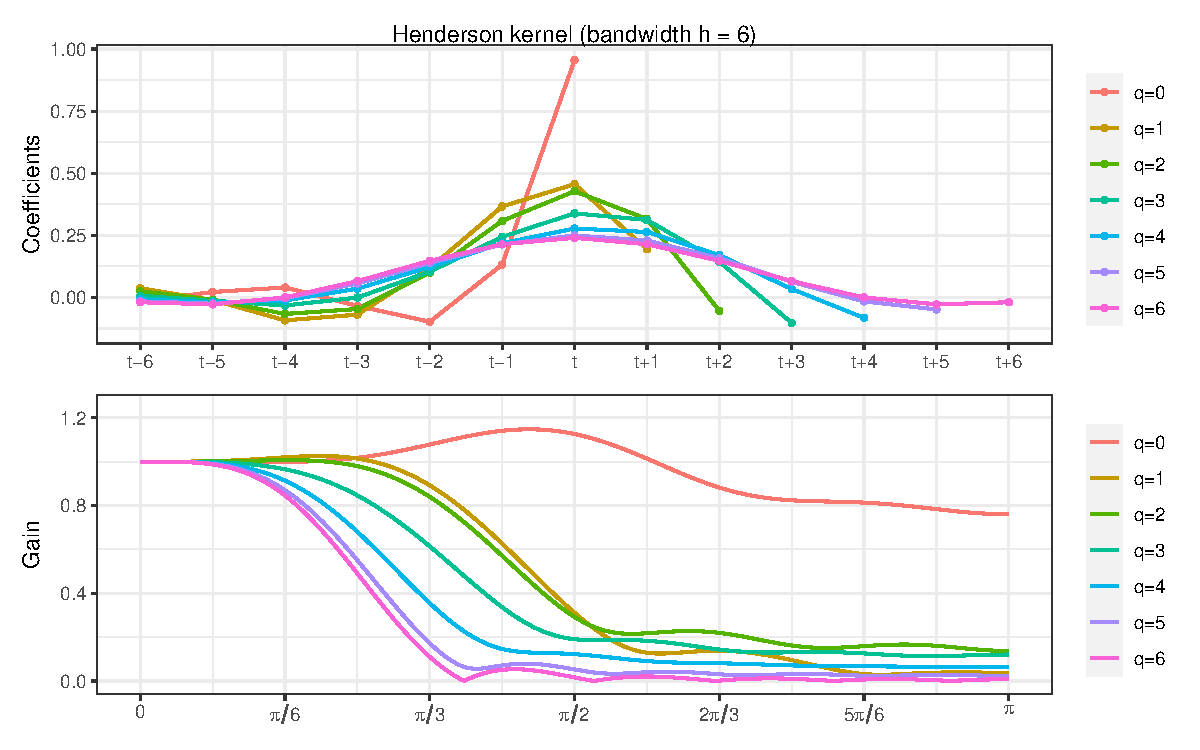
\includegraphics[width=\textwidth]{img/daf/coef_gain_1}
\caption{Coefficients and gain function of direct asymmetric filters (DAF) computed by local polynomial of degree $3$ with the Henderson kernel for $h=6$.}\label{fig:filtersdafcoefs}\footnotesize
\end{figure}

For all the kernels, we find the same results as in \textcite{proietti2008}:

\begin{itemize}
\item
  For a fixed value of \(d\), the more the data is available (\(q\) increases), the more the weight associated to the current observation \(w_{a,0}\) decreases.
\item
  For a fixed value of \(h\) and \(q\), \(w_{a,0}\) increases exponentially with the polynomial degree \(d\) (in particular, for \(d=h\), \(w_{a,0}=1\)).
\end{itemize}

\hypertarget{subsec:lppasymf}{%
\subsubsection{General class of asymmetric filters}\label{subsec:lppasymf}}

To deal with the problem of the variance of the estimates of the real-time filters, \textcite{proietti2008} suggest a general of asymmetric filters to make a tradeoff between bias and variance.

Here we consider that the data is generated by the model:
\[
y=U\gamma+Z\delta+\varepsilon,\quad
\varepsilon\sim\mathcal{N}(0,D)
\]
The goal is to find a filter \(v\) which minimize the mean square revision error (with the symmetric filter \(w\)) subject to some constraints.
The constraints are summarized by the matrix \(U=\begin{pmatrix}U_{p}'&U_{f}'\end{pmatrix}'\) (with \(U_p\) the available observations of the matrix \(U\) for the asymmetric filter): \(U_p'v=U'w\).
The problem is equivalent to find \(v\) that minimize:
\begin{equation}
\varphi(v)=
\underbrace{
  \underbrace{(v-w_{p})'D_{p}(v-w_{p})+
  w_{f}'D_{f}w_{f}}_\text{revision error variance}+
  \underbrace{[\delta'(Z_{p}'v-Z'w)]^{2}}_{biais^2}
}_\text{Mean square revision error}+
\underbrace{2l'(U_{p}'v-U'w)}_{\text{constraints}}
\label{eq:lppasym}
\end{equation}
with \(l\) a vector of Lagrange multipliers.

When \(U=X\) this is equivalent to the constraint to preserve polynomial of degree \(d\): we find the direct asymmetric filters \(w_a\) with \(D=K^{-1}\).

When \(U=\begin{pmatrix}1&\cdots&1\end{pmatrix}'\), \(Z=\begin{pmatrix}-h&\cdots&+h\end{pmatrix}'\), \(\delta=\delta_1\), \(D=\sigma^2I\) and when the symmetric filter is the Henderson filter we obtain the Musgrave asymmetric filters (used in the seasonal adjustment algorithm X-12ARIMA, see \textcite{musgrave1964set}).
With the filter we assume that the data is generated by a linear process and that the asymmetric filters preserve constant signals (\(\sum v_i=\sum w_i=1\)).
The asymmetric filters depends on the ratio \(\delta_1/\sigma\), which is related to the ``I-C'' ratio \(R=\frac{\bar{I}}{\bar{C}}=\frac{\sum\lvert I_t-I_{t-1}\rvert}{\sum\lvert C_t-C_{t-1}\rvert}\) (\(\delta_1/\sigma=2/(R\sqrt{\pi})\)), the ratio between the expected absolute difference of the irregular and of the trend-cycle.
In the seasonal adjustment method, the I-C ratio\footnote{To compute the I-C ratio, a first decomposition of the seasonally adjusted series is computed using a 13-term Henderson moving average.} is used to determine the bandwidth to used for the Henderson filter. For monthly data:

\begin{itemize}
\item
  if \(R<1\) a 9-term Henderson is used (\(h=4\));
\item
  if \(1\leq R\leq3.5\) a 13-term Henderson is used (\(h=6\));
\item
  if \(3.5< R\) a 23-term Henderson is used (\(h=12\)).
\end{itemize}

In this report, for simplicity we only consider 13-term symmetric filters: the ratio \(\delta^2/\sigma^2\) is fixed to \(3.5\).

When \(U\) corresponds to the first \(d^*+1\) first the columns of \(X\), \(d^*<d\), the constraint is that the asymmetric filter should reproduce polynomial of degree \(d^*\), the potential bias depends on the value of \(\delta\).
This will reduce the variance at the expense of a bias: it is the idea followed by \textcite{proietti2008} to propose three class of asymmetric filters:

\begin{enumerate}
\def\labelenumi{\arabic{enumi}.}
\item
  \emph{Linear-Constant} (LC): \(y_t\) linear (\(d=1\)) and \(v\) preserve constant signals (\(d^*=0\)).
  We obtain Musgrave filters when the Henderson kernel is used.
\item
  \emph{Quadratic-Linear} (QL): \(y_t\) quadratic (\(d=2\)), \(v\) depend on the ratio \(\delta_2^2/\sigma^2\).
\item
  \emph{Cubic-Quadratic} (CQ): \(y_t\) cubic (\(d=3\)), \(v\) depend on the ratio \(\delta_2^2/\sigma^2\).
\end{enumerate}

The table \ref{tab:criteriaLp} show the quality criteria of the different methods with the Henderson kernel and \(h=6\).
For real-time filters (\(q=0\)), the more complex the filter is (in terms of polynomial preservation), the less the timeliness is and the more the fidelity/smoothness is:the reduction of the time-delay is at the expense of an increase variance.
This change when \(q\) increases: for \(q=2\) the QL filter has a greater timeliness that the LC filter.
This unexpected result underlines the fact that in the approach of \textcite{proietti2008}, the timeliness is never set as a goal to minimize.

\begin{table}[!h]

\caption{\label{tab:criteriaLp}Quality criteria of asymmetric filters ($q=0,1,2$) computed by local polynomial with Henderson kernel for $h=6$ and $R=3.5$.}
\centering
\resizebox{\linewidth}{!}{
\begin{tabular}[t]{ccccccccccc}
\toprule
Method & $ b_c $ & $ b_l $ & $ b_q $ & $ F_g $ & $ S_g $ & $ T_g \times 10^{-3} $ & $ A_w $ & $ S_w $ & $ T_w $ & $ R_w $\\
\midrule
\addlinespace[0.3em]
\multicolumn{11}{l}{\textbf{$ q=0 $}}\\
\hspace{1em}LC & 0 & -0.407 & -2.161 & 0.388 & 1.272 & 30.341 & 0.098 & 0.488 & 0.409 & 0.548\\
\hspace{1em}QL & 0 & 0.000 & -0.473 & 0.711 & 5.149 & 0.047 & 0.067 & 1.894 & 0.000 & 0.106\\
\hspace{1em}CQ & 0 & 0.000 & 0.000 & 0.913 & 11.942 & 0.015 & 0.016 & 2.231 & 0.000 & 0.102\\
\hspace{1em}DAF & 0 & 0.000 & 0.000 & 0.943 & 14.203 & 0.003 & 0.015 & 2.178 & 0.000 & 0.098\\
\addlinespace[0.3em]
\multicolumn{11}{l}{\textbf{$ q=1 $}}\\
\hspace{1em}LC & 0 & -0.121 & -0.525 & 0.268 & 0.433 & 4.797 & 0.009 & 0.119 & 0.063 & 0.112\\
\hspace{1em}QL & 0 & 0.000 & -0.061 & 0.287 & 0.707 & 0.694 & 0.005 & 0.192 & 0.007 & 0.042\\
\hspace{1em}CQ & 0 & 0.000 & 0.000 & 0.372 & 0.571 & 0.158 & 0.022 & 0.575 & 0.001 & 0.061\\
\hspace{1em}DAF & 0 & 0.000 & 0.000 & 0.409 & 0.366 & 0.061 & 0.020 & 0.760 & 0.000 & 0.059\\
\addlinespace[0.3em]
\multicolumn{11}{l}{\textbf{$ q=2 $}}\\
\hspace{1em}LC & 0 & 0.003 & 1.076 & 0.201 & 0.080 & 0.347 & 0.009 & 0.012 & 0.004 & 0.015\\
\hspace{1em}QL & 0 & 0.000 & 0.033 & 0.215 & 0.052 & 2.083 & 0.000 & 0.011 & 0.023 & 0.067\\
\hspace{1em}CQ & 0 & 0.000 & 0.000 & 0.370 & 0.658 & 0.131 & 0.021 & 0.558 & 0.001 & 0.055\\
\hspace{1em}DAF & 0 & 0.000 & 0.000 & 0.398 & 0.768 & 0.023 & 0.017 & 0.677 & 0.000 & 0.048\\
\bottomrule
\end{tabular}}
\end{table}

Regarding the mean square revision error (\(A_w+S_w+T_w+R_w\)), LC and QL filters always gives better results than CQ and DAF filters.
This ``theorical'' mean square revision error can be compared to the ``empirical'' one computed applying the filters to real data.
The table \ref{tab:mseIPI} shows the average mean square revision error of the different filters applied to the Industrial production indices of the European Union between 2003 and 2019.
The mean square revision errors are different in level but give sames results comparing the different filters: this validate the formula used for the criteria \(A_w,S_w,T_w,\text{ and }R_w\) (see section \ref{sec:WildiMcLeroy}).

Taking for the value \(R\) the ``I-C'' ratio computed with the raw data gives the same summary results.

\begin{table}[!htb]
\caption{\label{tab:mseIPI}Mean square revision error of asymmetric filters ($q=0,1,2$) computed by local polynomial on the Industrial production indices of the European Union.}
\centering
\begin{tabular}[t]{cccc}
\toprule
\multicolumn{1}{c}{ } & \multicolumn{2}{c}{Mean squared revision error} & \multicolumn{1}{c}{ } \\
\cmidrule(l{3pt}r{3pt}){2-3}
Method & 2007-2010 & 2003-2019 & $A_w+S_w+T_w+R_w$\\
\midrule
\addlinespace[0.3em]
\multicolumn{4}{l}{\textbf{0}}\\
\hspace{1em}LC & 1.54 & 0.855 & 1.543\\
\hspace{1em}QL & 2.04 & 1.560 & 2.068\\
\hspace{1em}CQ & 2.88 & 2.363 & 2.349\\
\hspace{1em}DAF & 3.03 & 2.489 & 2.290\\
\addlinespace[0.3em]
\multicolumn{4}{l}{\textbf{1}}\\
\hspace{1em}LC & 2.96 & 1.315 & 0.304\\
\hspace{1em}QL & 2.31 & 1.074 & 0.247\\
\hspace{1em}CQ & 2.62 & 1.342 & 0.660\\
\hspace{1em}DAF & 2.72 & 1.437 & 0.840\\
\addlinespace[0.3em]
\multicolumn{4}{l}{\textbf{2}}\\
\hspace{1em}LC & 6.78 & 2.774 & 0.040\\
\hspace{1em}QL & 7.45 & 3.074 & 0.101\\
\hspace{1em}CQ & 7.99 & 3.620 & 0.635\\
\hspace{1em}DAF & 7.94 & 3.618 & 0.742\\
\bottomrule
\end{tabular}
\emph{Note: the filters are computed with $h=6$ (13-terms symmetric filter) and $R=3.5$.}
\end{table}

\faArrowCircleRight{} All those results suggest to focus on LC and QL filters and to focus on asymmetric linear filters that preserve polynomial trends of degree less than one.

The results for the different kernels can also be visualised in an online application available at \url{https://aqlt.shinyapps.io/FiltersProperties/}.

\begin{summary}{Local polynomial filters}

\textbf{Advantages}:

\begin{itemize}
\item
  Simple models with an easy interpretation.
\item
  The asymmetric linear filter is independent of the data and of the date of estimation.
\end{itemize}

\textbf{Drawbacks}:

\begin{itemize}
\tightlist
\item
  Timeliness is not controlled.
\end{itemize}

\end{summary}

\hypertarget{sec:GuggemosEtAl}{%
\section{\texorpdfstring{General optimisation problem: \textcite{ch15HBSA}}{General optimisation problem: @ch15HBSA}}\label{sec:GuggemosEtAl}}

\hypertarget{fst-filters}{%
\subsection{FST filters}\label{fst-filters}}

\textcite{ch15HBSA} defined a general approach to derive linear filters, based on an optimization problem of three criteria:

\begin{itemize}
\item
  \emph{Fidelity}, \(F_g\): it's the variance reduction ratio. It is called ``Fidelity'' because we want the output signal to be as close as possible to the input signal where the noise component is removed
  \[
  F_g(\theta) = \sum_{k=-p}^{+f}\theta_{k}^{2}
  \]
  \(F_g\) can be rewritten in a positive quadratic form: \(F_g(\theta)=\theta'F\theta\) with \(F\) the identity matrix of order \(p+f+1\).
\item
  \emph{Smoothness}, \(S_g\): it's the Henderson smoothness criterion (sum of the squared of the third difference of the coefficients of the filter).
  It measures the flexibility of the coefficient curve of a filter and the smoothness of the trend.
  \[
  S_g(\theta) = \sum_{j}(\nabla^{3}\theta_{j})^{2}
  \]
  \(S_g\) could also be rewritten in a positive quadratic form: \(S_g(\theta)=\theta'S\theta\) with \(S\) a symmetric matrix of order \(p+f+1\).
\item
  \emph{Timeliness}, \(T_g\): it measures the phase-shift between input and output signal for specific frequencies.
  When a linear filter is applied, the level input signal is also altered by the gain function.
  Therefore, it is natural to consider that the higher the gain is, the higher the phase shift impact is.
  That's why the timeliness criterion depends on the gain and phase shift functions (\(\rho_\theta\) and \(\varphi_{\theta}\)), the link between both functions being made by a penalty function \(f\).
  \[
  T_g(\theta)=\int_{\omega_{1}}^{\omega_{2}}f(\rho_{\theta}(\omega),\varphi_{\theta}(\omega))\ud\omega
  \]
  In this article we use \(\omega_1=0\) and \(\omega_2=2\pi/12\) (for monthly data): we focus on the phase shift impact on cycles of more than one year.
  For the penalty function, we take \(f\colon(\rho,\varphi)\mapsto\rho^2\sin(\varphi)^2\).
  Indeed, for this function, the timeliness criterion is analytically solvable (\(T_g=\theta'T\theta\) with \(T\) a square symmetric matrix of order \(p+f+1\)), which is better in a computational point of view.
\end{itemize}

The asymmetric filters are computed minimizing a weighted sum of the past three criteria, subject to some constraints. Those constraints are usually polynomial preservation.

\[
\begin{cases}
\underset{\theta}{\min} & J(\theta)=
\alpha F_g(\theta)+\beta S_g(\theta)+\gamma T_g(\theta)\\
s.t. & C\theta=a
\end{cases}
\]
The conditions \(\alpha,\beta,\gamma\geq 0\text{ and }\alpha+\beta\ne 0\) guarantee that \(J(\theta)\) is a strictly convex function: therefore the optimization problem has a unique solution.

The Henderson symmetric filters can for example be computed with
\[C=\begin{pmatrix}
1 & \cdots&1\\
-h & \cdots&h \\
(-h)^2 & \cdots&h^2
\end{pmatrix},\quad
a=\begin{pmatrix}
1 \\0\\0
\end{pmatrix},\quad
\alpha=\gamma=0,\quad
\beta=1\]

This approach can be called as the ``FST approach'' in reference to the three indicators used in the optimization problem.

\begin{summary}{FST filters}

\textbf{Advantages}:

\begin{itemize}
\item
  The asymmetric linear filter is independent of the symmetric filter, the data and the date of estimation.
\item
  Unique solution to the optimization problem.
\item
  The approach can be customized adding new criteria.
\end{itemize}

\textbf{Drawbacks}:

\begin{itemize}
\tightlist
\item
  The different criteria are not normalized: the associated weights cannot be compared.
\end{itemize}

\end{summary}

\hypertarget{extension-with-the-revision-criteria}{%
\subsection{Extension with the revision criteria}\label{extension-with-the-revision-criteria}}

The FST --- Fidelity-Smoothness-Timeliness --- approach is the only one that do not directly include a criterion on the revision error relative to a symmetric filter.\\
This approach could be somewhat generalized in order to include the revision criterion, replacing in the orthogonal form \(\theta\) by \((w-\theta)\) (with \(w\) the symmetric filter), and \(F\) by a matrix relative to the data (see \textcite{ch12HBSA}).

In this paper, we consider the method that consist to extend the minimization problem of local polynomial filters adding the Timeliness criteria defined by \textcite{ch15HBSA}\footnote{This method is for example coded in Java by Jean Palate in \url{https://github.com/palatej/jdemetra-core}.}.
Using the same notations as in section \ref{subsec:lppasymf}, \(\theta=v\) and noting \(g=v-w_p\), the Timeliness criterion can be rewritten:
\[
T_g(v)=v'Tv=g'Tg+2w_p'Tg+w_p'Tw_p
\quad(T\text{ being symmetric)}
\]
Moreover, the objective function \(\varphi\) of equation \eqref{eq:lppasym} can be rewritten as:
\begin{align*}
\varphi(v)&=(v-w_{p})'D_{p}(v-w_{p})+
  w_{f}'D_{f}w_{f}+
  [\delta'(Z_{p}'v-Z'w)]^{2}+
2l'(U_{p}'v-U'w)\\
&=g'Qg-2Pg+2l'(U_{p}'v-U'w)+c\quad\text{with }
\begin{cases}
Q=D_p+Z_p\delta\delta'Z'_p \\
P=w_fZ_f\delta\delta'Z_p'\\
c\text{ a constant independent of }v
\end{cases}
\end{align*}

Adding the Timeliness criteria, it becomes:
\[
\widetilde\varphi(v)=g'\widetilde Qg-
2\widetilde Pg+2l'(U_{p}'v-U'w)+
\widetilde c\quad\text{with }
\begin{cases}
\widetilde Q=D_p+Z_p\delta\delta'Z'_p +\alpha_TT\\
\widetilde P=w_fZ_f\delta\delta'Z_p'-\alpha_Tw_pT\\
\widetilde c\text{ a constant independent of }v
\end{cases}
\]
where \(\alpha_T\) is the weight associated to the Timeliness criterion. With \(\alpha_T=0\) we find \(\varphi(v)\).

The figures \ref{fig:lppguglc} show the impact of \(\alpha_T\) on the coefficients of the linear filter with the LC method:

\begin{itemize}
\item
  The more \(\alpha_T\) the more the coefficient associated to the current observation increases: this is what we expected.
\item
  The \(\alpha_T\) impact logarithmically the coefficients: we can restraint \(\alpha_T\) to \([0,2000]\).
\item
  As expected, to include the timeliness criteria has more impact for the value of \(q\) that gives filters with higher timeliness: it corresponds to \(q\leq2\) for the LC method. For the QL method we find thant \(\alpha_T\) has an impact for medium values of \(q\) (\(2\leq q\leq4\)).
\end{itemize}

\begin{figure}[!ht]
\animategraphics[autoplay,loop,width=\textwidth,controls]{0.5}{img/lppgug_lc_q}{0}{5} 
\caption{Impact of the timeliness weight ($\alpha_T$) on the coefficients of the local polynomial filter with the LC method with $h=6$, $R=3.5$ and the Henderson kernel.
}\label{fig:lppguglc}\footnotesize
\emph{Note: to see the animation, the PDF must be open with Acrobat Reader, KDE Okular, PDF-XChange or Foxit Reader. 
Otherwise you will only be able to see the results for $q=0$.}
\end{figure}

\hypertarget{sec:WildiMcLeroy}{%
\section{\texorpdfstring{Data-dependent filter: \textcite{trilemmaWMR2019}}{Data-dependent filter: @trilemmaWMR2019}}\label{sec:WildiMcLeroy}}

In \textcite{trilemmaWMR2019}, the authors proposed a data-dependent approach to derive linear filters. They decompose the mean square revision error in a trilemma between three quantities : \emph{accuracy}, \emph{timeliness} and \emph{smoothness}.

Let:

\begin{itemize}
\item
  \(\left\{ x_{t}\right\}\) be our input time series;
\item
  \(\left\{y_{t}\right\}\) the target signal, i.e.~the result of a symmetric filter, and \(\Gamma_s\), \(\rho_s\) and \(\varphi_s\) the associated frequency response, gain and phase shift functions.
\item
  \(\left\{\hat y_{t}\right\}\) an estimation of \(\left\{y_{t}\right\}\), i.e.~the result of an asymmetric filter (when not all observations are available), and \(\Gamma_\theta\), \(\rho_\theta\) and \(\varphi_\theta\) the associated frequency response, gain and phase shift functions.
\end{itemize}

If we assume that \(\left\{ x_{t}\right\}\) is weakly stationary with a continuous spectral density \(h\), the mean square revision error, \(\E{(y_{t}-\hat{y}_{t})^{2}}\), can be written as:
\begin{equation}
\E{(y_{t}-\hat{y}_{t})^{2}}=\frac{1}{2\pi}\int_{-\pi}^{\pi}\left|\Gamma_s(\omega)-{\Gamma_\theta}(\omega)\right|^{2}h(\omega)\ud\omega=\frac{1}{2\pi}\times2\times\int_{0}^{\pi}\left|\Gamma_s(\omega)-{\Gamma_\theta}(\omega)\right|^{2}h(\omega)\ud\omega
\label{eq:msedef}
\end{equation}

This equality can also be generalized to non-stationary integrated process (for example imposing cointegration between both signals and using pseudo-spectral density, see \textcite{optimrtfWMR2013}).

\begin{align}
\left|\Gamma_s(\omega)-\Gamma_\theta(\omega)\right|^{2} & =\rho_s(\omega)^{2}+\rho_\theta(\omega)^{2}+2\rho_s(\lambda)\rho_\theta(\lambda)\left(1-\cos(\varphi_s(\omega)-\varphi_\theta(\omega)\right) \nonumber\\
 & =\left(\rho_s(\omega)-\rho_\theta(\omega)\right)^{2}+4\rho_s(\lambda)\rho_\theta(\lambda)\sin^{2}\left(\frac{\varphi_s(\omega)-\varphi_\theta(\omega)}{2}\right)
 \label{eq:msedecomp}
\end{align}

The interval \([0,\pi]\) is then splitted in two: the pass-band \([0,\omega_1]\) (the frequency interval that contains the target signal) and the stop-band \([\omega_1,\pi]\).

The mean squared error defined in equation \eqref{eq:msedef} can then be decomposed additively into four quantities:
\begin{align*}
Accuracy =A_w&= 2\int_0^{\omega_1}\left(\rho_s(\omega)-\rho_\theta(\omega)\right)^{2}h(\omega)\ud\omega\\
Timeliness =T_w&= 8\int_0^{\omega_1}\rho_s(\lambda)\rho_\theta(\lambda)\sin^{2}\left(\frac{\varphi_\theta(\omega)}{2}\right)h(\omega)\ud\omega\\
Smoothness =S_w&= 2\int_{\omega_1}^\pi\left(\rho_s(\omega)^{2}-\rho_\theta(\omega)\right)^{2}h(\omega)\ud\omega\\
Residual =R_w&= 8\int_{\omega_1}^\pi\rho_s(\lambda)\rho_\theta(\lambda)\sin^{2}\left(\frac{\varphi_\theta(\omega)}{2}\right)h(\omega)\ud\omega\\
\end{align*}

\begin{remark}

The formulas of the four criteria slightly differ from the ones defined in \textcite{trilemmaWMR2019} to have coherent definitions between all sections:

\begin{itemize}
\item
  in this paper the interval integrations is \([0,\pi]\) rather than \([-\pi;\pi]\) (the integral are then only multiplied by 2 because all the functions are even);
\item
  the pass-pand interval is defined as the frequency interval that contains the target signals whereas in \textcite{trilemmaWMR2019} it depends on the gain function of the symmetric filer (pass-band\(=\{\omega |\rho_s(\omega)\geq 0.5\}\)).
\end{itemize}

\end{remark}

In general, the residual \(R_w\) is small since \(\rho_s(\omega)\rho_\theta(\omega)\) is close to 0 in the stop-band.
Moreover, user priorities are rarely concerned about the time-shift properties of components in the stop-band.
That's why, to derive linear filters the residual is not taken into account and that the authors suggest to compute then minimizing a weighted sum of the first three indicators:
\[
\mathcal{M}(\vartheta_{1},\vartheta_{2})=\vartheta_{1}T_w(\theta)+\vartheta_{2}S_w(\theta)+(1-\vartheta_{1}-\vartheta_{2})A_w(\theta)
\]
One of the drawbacks of this method is that there is no guarantee that there is a unique solution.

In this paper we focus in non-parametric approaches to derive linear filters.
That's why this approach is not considered.
However, the decomposition of the mean squared error gave useful indicators to compare linear filters because, in contrary the one presented in section \ref{sec:GuggemosEtAl}, their values can be easily interpreted and compared to each other.

To have criteria that don't depend on the data, we take for the symmetric filter the Henderson filter and we fix the spectral density to the one of a random walk:
\[
h_{RW}(x)=\frac{1}{2(1-\cos(x))}
\]
The formula presented in table \ref{tab:QC} are then found using the fact that for a symmetric filter the phase shit is equal to zero (\(\varphi_s(\omega)=0\)).

\begin{summary}{Data-dependent filters}

\textbf{Advantages}:

\begin{itemize}
\tightlist
\item
  The values of the different criteria can be compared: the weight can be easily interpreted.
\end{itemize}

\textbf{Drawbacks}:

\begin{itemize}
\item
  Data-dependent filter: it depends on the symmetric filter, the data and the date of estimation.
\item
  Some optimisation problems might occur (several minimum, etc.).
\end{itemize}

\end{summary}

\hypertarget{sec:Dagum}{%
\section{Asymmetric filters and Reproducing Kernel Hilbert Space}\label{sec:Dagum}}

\textcite{dagumbianconcini2008} developed a general approach to derive linear filters based on Reproducing Kernel Hilbert Space (RKHS) methodology.

A RKHS is a Hilbert space characterized by a kernel that reproduces, via an inner product defined by a density function \(f_0(t)\), every function of the space.
Therefore, a kernel estimator \(K_p\) of order \(p\) (i.e.~: that reproduce without distortion a polynomial trend of degree \(p-1\)) can be decomposed into the product of a reproducing kernel \(R_{p-1}\), belonging to the space of polynomials of degree \(p-1\), and a probability density function \(f_0\).

For any sequence \(\left(P_{i}\right)_{0\leq i\leq p-1}\) of orthonormal polynomials in \(\mathbb{L}^{2}(f_{0})\)\footnote{\(\mathbb{L}^{2}(f_{0})\) is the Hilbert space defined by the inner product:
  \[
  \left\langle U(t),V(t)\right\rangle =\E{U(t)V(t)}=\int_{\R}U(t)V(t)f_{0}(t)\ud t
  \]}, the kernel estimator \(K_p\) is defined by:
\[
K_{p}(t)=\sum_{i=0}^{p-1}P_{i}(t)P_{i}(0)f_{0}(t)
\]
The weight of a symmetric filter are then derived with:
\[
\forall j\in\left\llbracket -h,h\right\rrbracket\::\: w_{j}=\frac{K_p(j/b)}{\sum_{i=-h}^{^h}K_p(i/b)}
\]
where \(b\) is a time-invariant global bandwidth parameter.

The density \(f_0\) corresponds to the continuous versions of the kernel defined in \ref{sec:kernels}.
For example, the biweight function is \(f_{0B}(t)=(15/16)(1-t^2)^2,t\in [-1,1]\).
The local polynomial filter obtained with the biweight kernel is then obtained using the bandwidth \(b=m+1\).

The goal of \textcite{dagumbianconcini2008} is to derive asymmetric filters from the Henderson symmetric filter, therefore the ideal kernel function would be the Henderson one.
However, as shown in section \ref{sec:kernels}, the Henderson density is a function of the bandwidth and needs to be calculated any time \(m\) changes (as its corresponding orthonormal polynomial). That's why the authors use the biweight kernel to approximate the Henderson kernel (for \(h\geq 24\) they suggest to consider the triweight kernel).

The asymmetric weighted are obtained adapting the kernels to the length of the asymmetric filters:
\[
\forall j\in\left\llbracket -h,p\right\rrbracket\::\: w_{a,j}=\frac{K_p(j/b)}{\sum_{i=-h}^{^p}K_p(i/b)}
\]
With \(b=h+1\), \textcite{proietti2008} show that we obtain the direct asymmetric filters (DAF).

In \textcite{dagumbianconcini2015}, the authors suggest to perform an optimal bandwidth selection (parameter \(b\)), decomposing the mean squared revision error as in equation \eqref{eq:msedecomp} but with a uniform spectarl density (\(h(\omega)=1\)).
The bandwidth can then be chosen to minimize the mean squared revision error, the phase shift, etc.
The following bandwidth selection are studied:
\begin{align*}
b_{q,G}&=\underset{b_q\in]h;2 h+1]}{\min}
\sqrt{2\int_{0}^{\pi}
\left(\rho_s(\omega)-\rho_\theta(\omega)\right)^{2}\ud \omega
}\\
b_{q,\gamma}&=\underset{b_q\in]h;2 h+1]}{\min}
\sqrt{2\int_{0}^{\pi}
\lvert \Gamma_s(\omega)-\Gamma_\theta(\omega)\rvert^2\ud \omega
} \\
b_{q,\varphi}&=\underset{b_q\in]h;2 h+1]}{\min}
8\int_{0}^{2\pi/12}
\rho_s(\lambda)\rho_\theta(\lambda)\sin^{2}\left(\frac{\varphi_\theta(\omega)}{2}\right)\ud \omega
\end{align*}

One of the drawbacks of the optimal bandwidth selection is that there is no guarantee that there is a unique solution.

\begin{remark}

The formulas of \(b_{q,G}\), \(b_{q,\gamma}\) and \(b_{q,\varphi}\) slightly differ from the ones defined in \textcite{dagumbianconcini2015} to have coherent definitions between all sections:

\begin{itemize}
\tightlist
\item
  \(b_{q,\varphi}\) is defined as
  \[
  b_{q,\varphi}=\underset{b_q\in]h;2 h+1]}{\min}
  \sqrt{2\int_{\Omega_S}
  \rho_s(\lambda)\rho_\theta(\lambda)\sin^{2}\left(\frac{\varphi_\theta(\omega)}{2}\right)\ud \omega}
  \]
\end{itemize}

With \(\Omega_S=[0,2\pi/36]\) the frequency domain associated to cycles of 16 months or longer.

\begin{itemize}
\tightlist
\item
  in \textcite{dagumbianconcini2015} a different formula is used for the frequency response function (\(\Gamma_\theta(\omega)=\sum_{k=-p}^{+f} \theta_k e^{2\pi i \omega k}\)), it only changes the interval integration.
\end{itemize}

\end{remark}

The table \ref{tab:criteriarkhs} shows the quality criteria of the RKHS filters.
Even if the symmetric filter preserve quadratic trends, this is not the case of the asymmetric filters: they only preserve constant trends.
The more data is available (i.e.: \(q\) increases), the less the asymmetric filters distort polynomial trends (for example, for \(q=2\), \(b_c\simeq0\)).

\begin{table}[!h]

\caption{\label{tab:criteriarkhs}Quality criteria of asymmetric filters ($q=0,1,2$) computed by the RKHS methodology $h=6$.}
\centering
\resizebox{\linewidth}{!}{
\begin{tabular}[t]{ccccccccccc}
\toprule
Method & $ b_c $ & $ b_l $ & $ b_q $ & $ F_g $ & $ S_g $ & $ T_g \times 10^{-3} $ & $ A_w $ & $ S_w $ & $ T_w $ & $ R_w $\\
\midrule
\addlinespace[0.3em]
\multicolumn{11}{l}{\textbf{$ q=0 $}}\\
\hspace{1em}$b_{q,\gamma}$ & 0 & -1.526 & 3.893 & 0.222 & 0.469 & 74.991 & 0.017 & 0.069 & 2.164 & 0.671\\
\hspace{1em}$b_{q,G}$ & 0 & -2.039 & 6.937 & 0.177 & 0.305 & 98.650 & 0.082 & 0.066 & 3.547 & 0.715\\
\hspace{1em}$b_{q,\varphi}$ & 0 & -0.614 & 0.033 & 0.381 & 1.204 & 23.323 & 0.019 & 0.549 & 0.451 & 0.356\\
\addlinespace[0.3em]
\multicolumn{11}{l}{\textbf{$ q=1 $}}\\
\hspace{1em}$b_{q,\gamma}$ & 0 & -0.516 & 0.992 & 0.226 & 0.303 & 14.386 & 0.002 & 0.047 & 0.313 & 0.170\\
\hspace{1em}$b_{q,G}$ & 0 & -0.923 & 2.880 & 0.189 & 0.248 & 27.386 & 0.039 & 0.036 & 0.786 & 0.213\\
\hspace{1em}$b_{q,\varphi}$ & 0 & -0.176 & 0.295 & 0.276 & 0.359 & 2.901 & 0.003 & 0.182 & 0.050 & 0.071\\
\addlinespace[0.3em]
\multicolumn{11}{l}{\textbf{$ q=2 $}}\\
\hspace{1em}$b_{q,\gamma}$ & 0 & 0.041 & 0.863 & 0.202 & 0.090 & 0.328 & 0.006 & 0.010 & 0.004 & 0.018\\
\hspace{1em}$b_{q,G}$ & 0 & -0.007 & 1.001 & 0.197 & 0.096 & 0.637 & 0.009 & 0.010 & 0.008 & 0.021\\
\hspace{1em}$b_{q,\varphi}$ & 0 & 0.105 & 0.820 & 0.215 & 0.077 & 0.064 & 0.003 & 0.025 & 0.005 & 0.010\\
\bottomrule
\end{tabular}}
\end{table}

\begin{summary}{RKHS filters}

\textbf{Advantages}:

\begin{itemize}
\tightlist
\item
  Filters that apply to irregular frequency series (for example with a lot of missing values) can easily be computed.
\end{itemize}

\textbf{Drawbacks}:

\begin{itemize}
\item
  The linear filters don't preserve polynomial trends of degree 1 or more.
\item
  Some optimisation problems might occur (several minimum, etc.).
\end{itemize}

\end{summary}

\hypertarget{comparison-of-the-different-filters}{%
\section{Comparison of the different filters}\label{comparison-of-the-different-filters}}

\hypertarget{comparison-with-the-fst-approach}{%
\subsection{Comparison with the FST approach}\label{comparison-with-the-fst-approach}}

The FST approach provides a useful tool to validate a method of construction of linear filter.
Indeed, a linear filter can be considered as suboptimal if we can find a set of weight for the FST approach that gives better results (in terms of fidelity, smoothness and timeliness) with the same (or higher) polynomial constraints.

For \(h=6\) (13-term symmetric filter), for the RKHS filters we find that:

\begin{itemize}
\item
  imposing that asymmetric filter preserve constants, the FST approach gives better results for all values of \(q\) for the filters computed with \(b_{q,G}\) and \(b_{q,\gamma}\), and for \(q\leq 3\) for the one computed with \(b_{q,\varphi}\).
\item
  imposing that asymmetric filter preserve linear trends, the FST approach gives better results for \(q\in[2,5]\) for the filters computed with \(b_{q,G}\) and \(b_{q,\gamma}\), and for \(q\in[2,4]\) for the one computed with \(b_{q,\varphi}\).
\end{itemize}

\faArrowCircleRight{} Therefore, the RKHS approach seems not to be the better approach to build asymmetric filters to apply to monthly regular data (i.e.~: data for which we usually use \(h=6\)).

For the local polynomial filters we find that:

\begin{itemize}
\item
  imposing that asymmetric filter preserve constants, the FST approach gives better results than the LC method for all values of \(q\).
  Adding the timeliness criteria allows to have better results than the FST approach for \(q=0,1\).
\item
  imposing that asymmetric filter preserve linear trends, the FST approach gives better results for \(q\in[2,5]\) for the LC and QL methods. Adding the timeliness criteria doesn't change the results.
\end{itemize}

\faArrowCircleRight{} In terms of quality criteria, local polynomial seems to perform better for real-time and one-period ahead filters (\(q=0,1\)).

Those comparisons can be seen in an online application available at \url{https://aqlt.shinyapps.io/FSTfilters/}.

\hypertarget{illustration-with-an-example}{%
\subsection{Illustration with an example}\label{illustration-with-an-example}}

In this section we compare the different asymmetric filters applying them to the French industrial production index of manufacture of motor vehicles, trailers and semi-trailers\footnote{This series is produced by INSEE, the French National Statistical Office and is available at \url{https://bdm.insee.fr/series/sdmx/data/SERIES_BDM/010537940}.}.
For simplicity, for the FST approach we only show an extreme filter example minimizing the phase shift by putting a large weight to the timeliness (\(\alpha = 0\), \(\beta = 1\), \(\gamma = 1000\)). For local polynomial filters, the Henderson kernel is used with \(R=3.5\).
The figure \ref{fig:cl2all} shows the results around a turning point (the economic crisis of 2009) and during ``normal cycles'' (between 2000 and 2008).

\begin{figure}[!ht]
\animategraphics[autoplay,loop,width=\textwidth,controls]{2}{img/illustration/illustration_}{1}{7}
\caption{Application of asymmetric filters to the French industrial production index of manufacture of motor vehicles, trailers and semi-trailers.}\label{fig:cl2all}\footnotesize
\emph{Note: The final trend is the one computed by a symmetric 13-terms Henderson filter}

\emph{To see the animation, the PDF must be open with Acrobat Reader, KDE Okular, PDF-XChange or Foxit Reader.
Otherwise you will only be able to see the results for the DAF filter.}
\end{figure}

For this example, in terms of time lag to detect the turning point of February 2009\footnote{A turning point (upturn) is defined to occur at time \(t\) if \(y_{t-k}\geq\cdots\geq y_{t-1}<y_t\leq y_{t+1}\leq\cdots y_{t+m}\).
  A downturn would be equivalently defined as a date \(t\) \(y_{t-k}\leq\cdots\leq y_{t-1}>y_t\geq y_{t+1}\geq\cdots y_{t+m}\).
  Following \textcite{Zellner1991}, \(k=3\) and \(m=1\) are chosen given the smoothness of the trend-cycle data. }, the DAF is the worst filters since it introduce a delay of one month until \(q=3\).
LC, QL, \(b_{q,\gamma}\) filters introduce a delay only for real-time filter (\(q=0\)) of one month except for the QL filter for which it is of two months.
Surprisingly, the FST filter that minimize the phase shift introduce a time lag for \(q=0\) and \(q=1\) (the upturn is detected earlier), whereas \(b_{q,\phi}\) doesn't introduce any time lag.

In terms of revision error, the DAF filters also give the worst results.
For real-time estimates (\(q=0\)), the LC and RKHS filters minimize the revision between 2000 and 2008 but when more data are available all the methods (except the DAF filters) give similar results.
As excepted, the QL filter minimize the revision around the turning point of 2009 since it is the only filter that preserve polynomial trends of degree 1.
The fact that, around the turning point, \(b_{q,\phi}\) performs better than the other RKHS filters can be explain by the fact that this filter distort less polynomial trends of degree 1 and 2 (\(b_l\) and \(b_q\) statistics are lower, table \ref{tab:criteriaLp}).

With this simple example we cannot generalize properties on the different asymmetric filters but it gives some leads to extend this study:

\begin{itemize}
\item
  minimize the timeliness doesn't imply earlier detection of turning points: more investigations on the timeliness criteria could be done;
\item
  accept some bias in polynomial trends preservation can lead to asymmetric filters that performs better in term of turning points detection;
\item
  for almost all the filters, there is no time lag to detect the turning points when two future observations are available and the different methods gives similar results.
  Therefore, it is pointless to optimize asymmetric filters when too much future observations are available.
\end{itemize}

Moreover, this example also illustrate that the different methods performs better than the DAF filters.
The real-time estimates methods that use this filter could be easily improved.
This is for example the case of STL (Seasonal-Trend decomposition based on Loess) seasonal adjustment method proposed by \textcite{cleveland90}.

\newpage

\hypertarget{conclusion}{%
\section{Conclusion}\label{conclusion}}

To sum up, several lessons can be learn from this study on asymmetric filters.

First, to build asymmetric filters there is no need to seek to preserve polynomial trends of degree more than 2: it introduces more bias in the detection of turning point with a low gain on the revision error.
Moreover, introduce a small bias in polynomial preservation can lead to filters that performs globally better, as we have shown with RKHS \(b_{q,\phi}\) filter with the French IPI of manufacture of motor vehicles, trailers and semi-trailers.

Second, focusing on the Fidelity-Smoothness-Timeliness criteria, the FST approach can lead to asymmetric filters that performs better than the other ones (local polynomials and RKHS).
More investigations should be done in that direction to understand when it performs better and if the improvement is statistically significant.

Third, all the methods have advantages and drawbacks and lots of degrees of freedom on the criteria used to build them.
Therefore, more studies should be done on the effects of this degrees of freedom to see how they impact the estimation and if we cannot simplify them, as it is done in the X-12ARIMA algorithm to choose the length of the Henderson filter.

Finally, the study on asymmetric filters should be focus on real-time estimates and when few future observations are available. Indeed, for monthly data, when two or more future observations are available, the different methods gives similar results and the gain to compute optimize filters is small.

This study could also be extended in many ways.
One lead could be to do more investigation on the length of the filters.
In most of studies on asymmetric filters, the asymmetric filter uses as many past observations as the symmetric filters. However, we could consider asymmetric filters that takes more past observations. Moreover, in this paper we have only focus on regular monthly data but we could have some issues with high frequency data and irregular data.
In addition to the problem of choosing the length of the filter, we could check if we find similar results as for short filters.

Another lead could be to study the impact of atypical points: in X-12ARIMA there is a strong correction of atypical points on the irregular before applying the filters to extract the trend.
This therefore prompts us to study what would be their impact on the estimation of trends and turning points, but also to explore new kinds of asymmetric filters based on robust methods.

\newpage

\printbibliography[title=References]

\end{document}
